% Standalone TikZ figure (compile to PDF/SVG for embedding in Markdown).
\documentclass[tikz,border=2pt]{standalone}
\usepackage{tikz}
\usetikzlibrary{positioning,arrows.meta}

\begin{document}
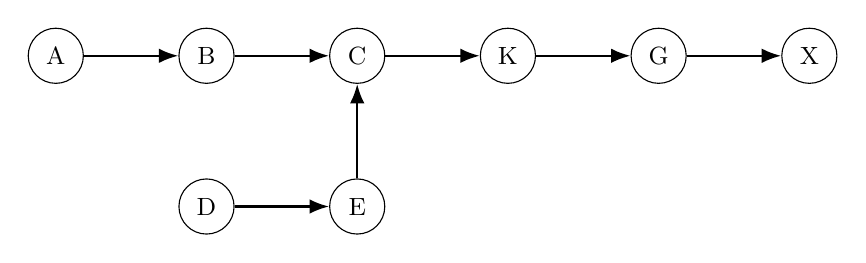
\begin{tikzpicture}[
  node/.style={draw, circle, minimum size=7mm, inner sep=0pt, font=\small},
  link/.style={line width=0.9pt},
  msg0/.style={-Latex, line width=1.1pt, blue},
  msg1/.style={-Latex, line width=1.1pt, teal!70!black},
  msg2/.style={-Latex, line width=1.1pt, orange!85!black},
  oneway/.style={-Latex, link}
]

% Nodes (top row)
\node[node] (A) {A};
\node[node, right=12mm of A] (B) {B};
\node[node, right=12mm of B] (C) {C};
\node[node, right=12mm of C] (K) {K};
\node[node, right=12mm of K] (G) {G};
\node[node, right=12mm of G] (X) {X};

% Nodes (bottom branch)
\node[node, below=12mm of C] (E) {E};
\node[node, left=12mm of E] (D) {D};

% Base connectivity (bidirectional/undirected links on the left)
\draw[oneway] (A) -- (B);
\draw[oneway] (B) -- (C);
\draw[oneway] (C) -- (K);

% One-way links to the right (so G/X can't reach K)
\draw[oneway] (K) -- (G);
\draw[oneway] (G) -- (X);

% Branch connectivity
\draw[oneway] (E) -- (C);
\draw[oneway] (D) -- (E);

\end{tikzpicture}
\end{document}
